\section{Übersicht}
\begin{enumerate}
  \item Defintion Ladung, Strom, Spannung, Potential
  \item Grundstromrkeis, Darstellung
  \item Widerstand $\Omega$ Ohmisches Gesetz
  \item Mehrteilige Schaltungen
  \begin{enumerate}[label*=\arabic*.]
    \item Stromknoten
    \item Spannungsmasche
    \item Superpostionsprinzip
  \end{enumerate}
  \item Reale Spannungs und Stromquellen
  \item Leistung
  \item Zeit abhänige Spannugen und Ströme
  \item Blindelement $L,C$
\end{enumerate}


\section{Elektronen}

Elektronische Ladung $Q$ besteht aus \underline{Elektronnen}\\
Stets \underline{negative} Ladung \\
(Postive Ladung ist Elektronenmangel, setzt Stoff vorraus)\\
1 Elektron hat eine Elementarladung von $e = 1,6 \cdot 10^{-19} A \cdot s$\\
\\
\\
$ Q = A \cdot s $ ($A/s$  Amper Sekunde) wegen negative: $q = -1,6 \cdot 10^{-19} A \cdot s$\\
\\
$Q_{Elektron} = -1,6 \cdot 10^{-19} A \cdot s$\\
Für úberschus\\
\\
\\
Eine Wolke hat eine Ladung von $Q_{wolke} = 1 As$\\
\\
$ Q = n * q$\\
$n$ ist die Anzahl der $E$\\
$n = ? $\\
\\
$n = \frac{Q}{q} = \frac{1 As}{-1,6 \cdot 10^{-19} As}$\\
\\
Wir können kürzen:\\
$\frac{1 \cancel{As}}{-1,6 \cdot 10^{-19} \cancel{As}}$\\
$\approx \frac{1}{-1,6} \cdot 10^{19}$\\
$\approx \frac{5}{8} \cdot 10^{19}$\\
\\

\section{Spannung}
\underline{Spannung ist ein Zustand}\\
platzhalter bild\\
Es herrscht eine \underline{Spannung $U$}\\
Oder Wolke 2\\
Platzhalter bild2\\
$ U > 0 $\\
\\

Wolke3\\
Platzhalter Bild3\\

Spannungsrichtung festlegung mit einem Zählpfeile (\underline{willkührliche Annahme})\\
hier Spannung von Erde zur Wolke \underline{positive}\\
\\
Einheit der Spannung\\
Volt, kurz $V$\\
\\
Angabe ziB $U = + 230 V \leftarrow $ Buchstabe als Einheit\\

\newpage

Vorsätze

$ 1 =1 $\\
$ 1000 = 10^3 = k $ (kilo)\\
Übersicht:\\
$ 10^{-12} = p $ ("pico")\\
$ 10^{-9} = n $ ("nano")\\
$ 10^{-6} = \mu $ ("mikro")\\
$ 10^{-3} = m $ ("milli")\\
$ 10^{-2} = c $ ("centi")\\
$ 10^{-1} = d $ ("deci")\\
$ 10^{1} = da $ ("deca")\\
$ 10^{2} = h $ ("hecto")\\
$ 10^{3} = k $ ("kilo")\\
$ 10^{6} = M $ ("mega")\\
$ 10^{9} = G $ ("giga")\\
$ 10^{12} = T $ ("tera")\\


\section{Strom}

\underline{Strom} ist die Bewegung von Elektronen. (d.h "Ladung fließt")

Gleichstrom, Konstanter Elektronenfluß.


\begin{figure}[h]
  \begin{center}
   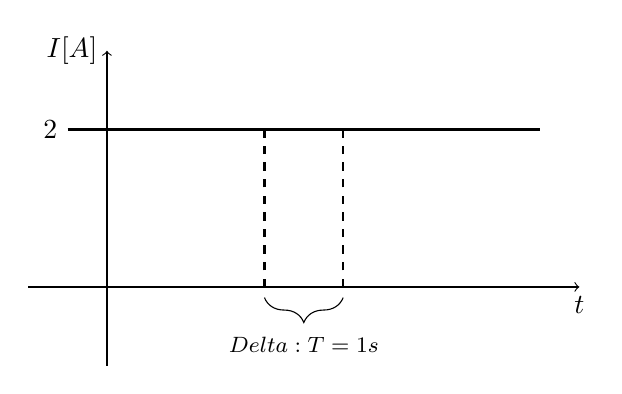
\begin{tikzpicture}
    \draw[->] (0,-1) -- (0,3) node[anchor=east] {$I [A]$};
    \draw[->] (-1,0) -- (6,0) node[anchor=north] {$t$};
    \draw[thick] (-0.5,2) node[anchor=east] {$2$}-- (5.5,2) ;
    \draw[thick,dashed] (2,0) -- (2,2);
    \draw[thick,dashed] (3,0) -- (3,2);
    \draw [decorate,decoration={mirror,brace,amplitude=9pt},yshift=-1pt](2,-0.1) -- (3,-0.1) node [black,midway,yshift=-0.6cm] {\footnotesize $Delta: T=1s$} ;
   \end{tikzpicture}
  \end{center}
\end{figure}

Aussage: Gleichstrom: $I = 2 \cdot A$\\
Zeit als ein interval\\
Zeit in Allgemeinen als Zeitabschnitt Benutzt, dann $T$\\
\\
Definition:\\
Strom $I$ ist fliesende Ladung $Q$ pro Zeit intervall $T$ damit $ I[A] = \frac{Q[A\cdot s]}{T[s]} $\\
Bespiel ergäbe:\\
$ Q = I \cdot T$\\
Wie = $2 A \cdot 1s  = \underline{2 As} $\\
Üblich: Kurzes Zeit intervall $\Delta T$\\
\\
$ I = \frac{\Delta Q}{\Delta T} \rightarrow \frac{d Q}{d t} $  
$ lim \Delta \rightarrow 0 $ \\
\\
Beschreiben von Strömlichen veränderung (nicht gleich Strom) diese Gleichung gilt auch für Zeit veränderliche Ströme.\\
\\
(Ableitung der Steigung nder der Zeit = Anstieg).\\
\begin{figure}[h]
  \begin{center}
   \begin{tikzpicture}
    \draw[->] (0,-1) -- (0,3) node[anchor=east] {$i(t)$};
    \draw[->] (-1,0) -- (6,0) node[anchor=north] {$t$};
    \draw[thick] (2,0) -- (2,2)-- (3,2) -- (3,0);
   \end{tikzpicture}
  \end{center}
\end{figure}
\\
\begin{figure}[h]
  \begin{center}
   \begin{tikzpicture}
    \draw[->] (0,-1) -- (0,3) node[anchor=east] {$Q$};
    \draw[->] (-1,0) -- (6,0) node[anchor=north] {$t$};
    \draw[thick] (2,0) -- (3,2) node[anchor=north] {Anstieg Konstant};
   \end{tikzpicture}
  \end{center}
\end{figure}\\
\\
Stromrichtung?\\
Platzhalter Bild Stromrichtung
\\
Elektronenfluß von lunks nach rechts.\\
Technische Richtung:\\
Platzhalter Bild Tech. Stromrichtung\\
\\
Konsequenz der historihscen Festlegung\\
Technisch gesehen hat die Spannung das Primat. Damit aus einem Spannung eine Stromfluß resultiert, muss eine Möglichkeit bestehen, meist ein \underline{Widerstand}.\\
\\
iderstand ist der Qocient aus Spannung und Strom:\\
Widerstand $R = \frac{Spannung U}{Strom I} $ Einheit $R[\Omega] = \frac{U[V]}{I[A]}$\\
\\
Kurz $ R = \frac{U}{I} $\\
$ 1\Omega = \frac{1V}{1A} $\\

